\chapter{The Greeks and Delta Hedging}
\label{ch:greeks_hedging}
\chaptermark{Greeks and delta hedging}

The Black--Scholes formula of \cref{ch:black_scholes} gives today's
call price, but in five minutes the underlying will have moved,
implied vol will have re-priced, and the option will have lost time
value. The \emph{Greeks} are the partial derivatives of the option
price with respect to the five inputs
$(\Spx,\,\volat,\,t,\,\rrf,\,\Kstrike)$, and every position on a
derivatives desk is booked, hedged, and risk-managed in terms of
its Greeks rather than its mark-to-market price \citeNatenberg.

This chapter has two goals. First, derive the closed-form Greeks
for a Black--Scholes European call --- delta, gamma, vega, theta,
rho --- pinned to the running example ($\Spx = \Kstrike = 100$,
$\rrf = 5\%$, $\volat = 20\%$, $\Tmat - t = 1$) from
\cref{ch:black_scholes}. Second, prove the P\&L identity behind
\emph{delta-hedging}: a delta-neutral long-option book makes money
when realised volatility exceeds implied and loses when it does
not. That gamma-against-theta identity is the central equation of
vol trading.

\begin{backgroundbox}[Prerequisites]
From earlier in the book:
\begin{itemize}
  \item \Cref{ch:options_payoffs}: European call and put payoffs,
  put--call parity, and the no-arbitrage bounds. Several Greeks
  inherit a parity-style call-versus-put relationship.
  \item \Cref{ch:black_scholes}: the Black--Scholes call price
  \begin{equation*}
    \Call \;=\; \Spx\,\CDFN(d_1) \;-\; \Kstrike\,e^{-\rrf(\Tmat-t)}\,\CDFN(d_2),
  \end{equation*}
  with $d_1 = [\ln(\Spx/\Kstrike) + (\rrf + \tfrac12 \volat^2)(\Tmat - t)]
  /(\volat\sqrt{\Tmat - t})$ and $d_2 = d_1 - \volat\sqrt{\Tmat - t}$;
  the Black--Scholes PDE
  $\Theta + \rrf \Spx\,\Delta + \tfrac12 \volat^2 \Spx^2\,\Gamma = \rrf\,\Call$;
  the running numerical example ($\Spx = \Kstrike = 100$, $\rrf =
  5\%$, $\volat = 20\%$, $\Tmat - t = 1$) which gives $d_1 = 0.35$,
  $d_2 = 0.15$, $\Call \approx 10.4506$.
  \item \Cref{ch:mean_reversion_ou}: It\^o's lemma in the form
  $df = f_t\,dt + f_x\,dX_t + \tfrac12 f_{xx}\,(dX_t)^2$ for an
  It\^o process $X_t$. The dynamic-hedging P\&L derivation re-uses
  this expansion.
\end{itemize}
From outside the book:
\begin{itemize}
  \item Multivariable calculus at the level of partial derivatives
  and the chain rule.
  \item The standard normal density $\pdfN(x) = (2\pi)^{-1/2}
  e^{-x^2/2}$ and CDF $\CDFN(x) = \int_{-\infty}^x \pdfN(u)\,du$.
\end{itemize}
\end{backgroundbox}

\begin{intuitionbox}
A Greek is a sentence the trader can speak: ``my book is long $+10{,}000$
delta of SPX, short $-50{,}000$ gamma, long $+200{,}000$ vega, and
bleeding $-30{,}000$ theta a day.'' Each number is the partial
derivative of the book's mark-to-market with respect to one input.
Together they tell the trader how the book will move as the world
moves --- and which parameter to hedge first. The Greeks are the
\emph{language} of risk on a derivatives desk.
\end{intuitionbox}

\section{The first-order Greeks: Delta and Rho}
\label{sec:ch16_first_order}

The five primary Greeks split into first-order sensitivities
(delta, rho, vega, theta) and second-order (gamma, plus
higher-order vanna/volga/charm). We start with the two simplest:
delta with respect to spot, rho with respect to interest rate.

\subsection{Delta: $\Delta = \partial \Call / \partial \Spx$}
\label{subsec:ch16_delta}

\begin{definition}[Delta]
\index{delta (Greek)|textbf}\index{Greeks!delta|textbf}
The \emph{delta} of an option price $V(\Spx, t)$ with respect to
its underlying $\Spx$ is the partial derivative
\begin{equation}
  \Delta \;\defeq\; \frac{\partial V}{\partial \Spx}.
  \label{eq:delta_def}
\end{equation}
For a European call price $\Call(\Spx, t)$ on a non-dividend-paying
stock under the Black--Scholes model, the delta is
\begin{equation}
  \Delta \;=\; \CDFN(d_1).
  \label{eq:delta_call}
\end{equation}
\end{definition}

The formula $\Delta = \CDFN(d_1)$ is one of the cleanest results in
derivatives, but it is not obvious from the call price
\begin{equation*}
  \Call(\Spx, t) \;=\; \Spx\,\CDFN(d_1) \;-\; \Kstrike\,e^{-\rrf(\Tmat - t)}\,\CDFN(d_2),
\end{equation*}
since both $d_1$ and $d_2$ depend on $\Spx$. Naive differentiation
produces four terms that must collapse. The same cancellation
reappears for vega, theta, and the vol-surface calibration of
\cref{ch:vol_surface}, so it is worth working once.

\paragraph{Derivation of $\Delta = \CDFN(d_1)$.}
Differentiate $\Call$ in $\Spx$ holding $t$, $\rrf$, $\volat$,
$\Kstrike$ fixed; let $\tau = \Tmat - t$. By product/chain rule,
\begin{align}
  \frac{\partial \Call}{\partial \Spx}
    \;&=\; \CDFN(d_1)
       \;+\; \Spx\,\pdfN(d_1)\,\frac{\partial d_1}{\partial \Spx}
       \;-\; \Kstrike\,e^{-\rrf \tau}\,\pdfN(d_2)\,\frac{\partial d_2}{\partial \Spx}.
  \label{eq:delta_derivation_step1}
\end{align}
Both $d_1$ and $d_2$ depend on $\Spx$ only through $\ln \Spx$, so
\begin{equation*}
  \frac{\partial d_1}{\partial \Spx}
  \;=\; \frac{\partial d_2}{\partial \Spx}
  \;=\; \frac{1}{\Spx\,\volat\sqrt{\tau}}.
\end{equation*}
So~\eqref{eq:delta_derivation_step1} reduces to
\begin{equation}
  \frac{\partial \Call}{\partial \Spx}
    \;=\; \CDFN(d_1)
       \;+\; \frac{1}{\volat\sqrt{\tau}}
              \Bigl[\,\pdfN(d_1) \;-\; \frac{\Kstrike}{\Spx}\,e^{-\rrf \tau}\,\pdfN(d_2)\,\Bigr].
  \label{eq:delta_derivation_step2}
\end{equation}
The bracket must vanish for~\eqref{eq:delta_call} to hold. The key
identity:
\begin{equation}
  \Spx\,\pdfN(d_1) \;=\; \Kstrike\,e^{-\rrf \tau}\,\pdfN(d_2),
  \label{eq:bs_identity}
\end{equation}
which we now prove. Take the ratio
\begin{align*}
  \frac{\Spx\,\pdfN(d_1)}{\Kstrike\,e^{-\rrf \tau}\,\pdfN(d_2)}
   \;&=\; \frac{\Spx}{\Kstrike}\,e^{\rrf \tau}\,
          \frac{e^{-d_1^2/2}}{e^{-d_2^2/2}}
   \;=\; \frac{\Spx}{\Kstrike}\,e^{\rrf \tau}\,
          \exp\!\Bigl(\,\tfrac{1}{2}(d_2^2 - d_1^2)\,\Bigr).
\end{align*}
Now $d_2^2 - d_1^2 = (d_2 - d_1)(d_2 + d_1) = (-\volat\sqrt\tau)
\,(2 d_1 - \volat\sqrt\tau)$, and substituting the explicit form of
$d_1$ gives
\begin{align*}
  \tfrac{1}{2}(d_2^2 - d_1^2)
   \;&=\; -\tfrac{1}{2}\,\volat\sqrt\tau\,
          \Bigl[\, 2 d_1 \;-\; \volat\sqrt\tau \,\Bigr] \\
   \;&=\; -\,\volat\sqrt\tau \cdot d_1 \;+\; \tfrac{1}{2}\,\volat^2\,\tau \\
   \;&=\; -\ln(\Spx/\Kstrike) \;-\; \rrf\,\tau,
\end{align*}
using $d_1 = [\ln(\Spx/\Kstrike) + (\rrf + \tfrac12\volat^2)\tau]
/(\volat\sqrt\tau)$; the emerging $-\tfrac12\volat^2\tau$ cancels
against the trailing $+\tfrac12\volat^2\tau$. Hence
\begin{equation*}
  \exp\!\Bigl(\,\tfrac{1}{2}(d_2^2 - d_1^2)\,\Bigr)
   \;=\; \frac{\Kstrike}{\Spx}\,e^{-\rrf \tau},
\end{equation*}
so the ratio collapses to $1$. This proves~\eqref{eq:bs_identity},
kills the bracketed term in~\eqref{eq:delta_derivation_step2}, and
leaves $\partial \Call / \partial \Spx = \CDFN(d_1)$. \citeHull
\S15.5 walks the same identity; it is the prototype for all
subsequent Greek derivations.

\begin{keyfactbox}[Delta of a Black--Scholes call]
\begin{equation*}
  \Delta_{\text{call}} \;=\; \frac{\partial \Call}{\partial \Spx}
   \;=\; \CDFN(d_1) \;\in\; (0, 1).
\end{equation*}
By put--call parity (\cref{ch:options_payoffs}),
$\Delta_{\text{put}} = \CDFN(d_1) - 1 \in (-1, 0)$. The call delta
is the share count replicating the call's instantaneous P\&L; the
put delta is negative because a put is a short directional
position.
\end{keyfactbox}

\paragraph{Delta as the replicating share count.}
The replicating-portfolio derivation of \cref{ch:black_scholes}
already met this number: the self-financing portfolio holds
$\CDFN(d_1)$ shares at time $t$. A trader long one call hedges by
\emph{shorting} $\Delta$ shares; short one call, by \emph{buying}
$\Delta$ shares. Either way the linear directional exposure is
zero and the position is \emph{delta-neutral}.

\paragraph{Delta by moneyness.} From $\Delta = \CDFN(d_1)$:
\begin{itemize}
  \item Deep \emph{in-the-money} call ($\Spx \gg \Kstrike$): $d_1
  \to +\infty$, $\Delta \to 1$. The call behaves like a forward on
  the stock.
  \item \emph{At-the-money} call ($\Spx \approx \Kstrike$), $d_1$
  small and positive, so $\Delta \approx 0.5$ --- the trader's rule
  of thumb ``ATM call delta is about a half''.
  \item Deep \emph{out-of-the-money} call ($\Spx \ll \Kstrike$):
  $d_1 \to -\infty$, $\Delta \to 0$. The call has almost no chance
  of being exercised.
\end{itemize}

\subsection{Worked numerical example: delta of the running call}
\label{subsec:ch16_delta_numex}

Take the running parameters of \cref{ch:black_scholes}:
$\Spx = \Kstrike = 100$, $\rrf = 5\%$, $\volat = 20\%$,
$\Tmat - t = 1$. The chapter calculation already gave
$d_1 = 0.35$ and $d_2 = 0.15$. Therefore
\begin{equation}
  \Delta \;=\; \CDFN(d_1) \;=\; \CDFN(0.35) \;\approx\; 0.6368.
  \label{eq:delta_numex}
\end{equation}
A trader long one call hedges by shorting $0.6368$ shares: $\$63.68$
of short stock against a $\$10.45$ option. The hedge exceeding the
premium is normal --- the delta-hedged position is a vol bet, and
most capital is tied up in the hedge.

\paragraph{Sanity check from the Ch~15 table.}
The comparative-statics table in \cref{ch:black_scholes} gave
$\Call = 5.09$ at $\Spx = 90$ and $\Call = 17.66$ at $\Spx = 110$.
The finite-difference slope is
\begin{equation*}
  \frac{17.66 - 5.09}{110 - 90} \;=\; \frac{12.57}{20} \;\approx\; 0.6285,
\end{equation*}
agreeing with the analytic $0.6368$ to two decimals. The gap is
central-difference truncation error from a $\$20$ secant step
across a curved function (the curvature is the gamma of the next
section).

\subsection{Rho: $\rho = \partial \Call / \partial \rrf$}
\label{subsec:ch16_rho}

\begin{keyfactbox}[Rho of a Black--Scholes call]
\begin{equation*}
  \rho_{\text{call}} \;=\; \frac{\partial \Call}{\partial \rrf}
   \;=\; \Kstrike\,(\Tmat - t)\,e^{-\rrf(\Tmat - t)}\,\CDFN(d_2).
\end{equation*}
Always positive: a higher discount rate raises the PV of the ITM
strike receipt. Put rho $\rho_{\text{put}} = -\Kstrike\,(\Tmat -
t)\,e^{-\rrf(\Tmat-t)}\,\CDFN(-d_2) < 0$.
\end{keyfactbox}

The derivation parallels delta. Differentiating
$\Call = \Spx\,\CDFN(d_1) - \Kstrike\,e^{-\rrf \tau}\,\CDFN(d_2)$
with respect to $\rrf$ produces contributions through $d_1$, $d_2$,
and the explicit $e^{-\rrf \tau}$ factor. Since $\partial d_1 /
\partial \rrf = \partial d_2 / \partial \rrf = \sqrt{\tau}/\volat$,
identity~\eqref{eq:bs_identity} again kills the bracketed piece,
leaving the explicit $\Kstrike\,\tau\,e^{-\rrf \tau}\,\CDFN(d_2)$
term. \citeHull \S17.10 has the full algebra.

\paragraph{Numerical value at the running parameters.} With
$\Kstrike = 100$, $\Tmat - t = 1$, $\rrf = 5\%$,
$e^{-\rrf \tau} = e^{-0.05} \approx 0.9512$, and
$\CDFN(d_2) = \CDFN(0.15) \approx 0.5596$,
\begin{equation*}
  \rho \;=\; 100 \cdot 1 \cdot 0.9512 \cdot 0.5596 \;\approx\; 53.23
  \quad \text{per unit of $\rrf$}.
\end{equation*}
By convention rho is reported per $1\%$ rate move ($\rrf \to \rrf
+ 0.01$), so $\rho/100 \approx 0.5323$: a one-percentage-point rate
increase raises the ATM one-year call by about $\$0.53$. Rho is
rarely the headline Greek for short-dated equity options; it
dominates long-dated rates products
(\cref{ch:rates_derivatives}).

\section{The second-order Greek: Gamma}
\label{sec:ch16_gamma}

If delta is the slope of the call price in spot, gamma is its
curvature. Gamma is the rate at which the delta hedge stops working,
and therefore the rate at which it must be rebalanced.

\begin{definition}[Gamma]
\index{gamma (Greek)|textbf}\index{Greeks!gamma|textbf}
The \emph{gamma} of an option price $V(\Spx, t)$ with respect to its
underlying $\Spx$ is the second partial derivative
\begin{equation}
  \Gamma \;\defeq\; \frac{\partial^2 V}{\partial \Spx^2}
                 \;=\; \frac{\partial \Delta}{\partial \Spx}.
  \label{eq:gamma_def}
\end{equation}
For a Black--Scholes European call on a non-dividend-paying stock,
\begin{equation}
  \Gamma \;=\; \frac{\pdfN(d_1)}{\Spx\,\volat\,\sqrt{\Tmat - t}}.
  \label{eq:gamma_call}
\end{equation}
\end{definition}

\paragraph{Derivation.} Differentiate $\Delta = \CDFN(d_1)$ with
respect to $\Spx$. By the chain rule,
\begin{equation*}
  \Gamma \;=\; \frac{d \CDFN(d_1)}{d d_1}\,\frac{\partial d_1}{\partial \Spx}
        \;=\; \pdfN(d_1)\,\cdot\,\frac{1}{\Spx\,\volat\,\sqrt{\tau}},
\end{equation*}
which is~\eqref{eq:gamma_call}. Gamma is positive for any long
option (call or put, by parity) since all factors are positive;
long options are \emph{long gamma}, short options are \emph{short
gamma}. Gamma scales like $1/(\Spx\,\volat\,\sqrt\tau)$, blowing up
close to expiry, on low-vol underlyings, and on low-priced
underlyings.

\begin{keyfactbox}[Gamma of a Black--Scholes call/put]
\begin{equation*}
  \Gamma \;=\; \frac{\pdfN(d_1)}{\Spx\,\volat\,\sqrt{\Tmat - t}} \;>\; 0.
\end{equation*}
By parity, calls and puts on the same strike/expiry have
\emph{identical} gamma. Long options are long gamma; short options
are short gamma.
\end{keyfactbox}

\begin{figure}[ht]
\centering
\begin{minipage}{0.48\textwidth}
\centering
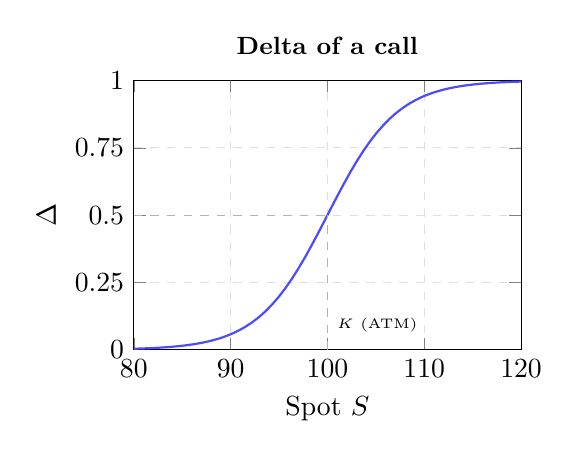
\begin{tikzpicture}
\begin{axis}[
  width=6.5cm, height=5cm,
  xlabel={Spot $S$},
  ylabel={$\Delta$},
  xmin=80, xmax=120,
  ymin=0, ymax=1,
  ytick={0,0.25,0.5,0.75,1},
  title={Delta of a call},
  title style={font=\small\bfseries},
  grid=major, grid style={dashed,gray!25},
]
\addplot[blue!70, thick, domain=80:120, samples=60]
  {1/(1+exp(-0.28*(x-100)))};
\addplot[dashed, gray!60, thin] coordinates {(100,0)(100,0.5)};
\addplot[dashed, gray!60, thin] coordinates {(80,0.5)(100,0.5)};
\node[font=\tiny, above right] at (axis cs:100,0.03) {$K$ (ATM)};
\end{axis}
\end{tikzpicture}
\end{minipage}
\hfill
\begin{minipage}{0.48\textwidth}
\centering
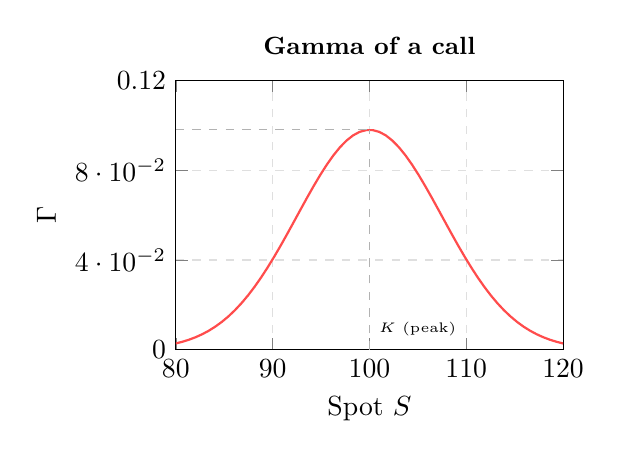
\begin{tikzpicture}
\begin{axis}[
  width=6.5cm, height=5cm,
  xlabel={Spot $S$},
  ylabel={$\Gamma$},
  xmin=80, xmax=120,
  ymin=0, ymax=0.12,
  ytick={0,0.04,0.08,0.12},
  title={Gamma of a call},
  title style={font=\small\bfseries},
  grid=major, grid style={dashed,gray!25},
]
\addplot[red!70, thick, domain=80:120, samples=60]
  {0.098*exp(-0.5*((x-100)/7.5)^2)};
\addplot[dashed, gray!60, thin] coordinates {(100,0)(100,0.098)};
\addplot[dashed, gray!60, thin] coordinates {(80,0.098)(100,0.098)};
\node[font=\tiny, above right] at (axis cs:100,0.002) {$K$ (peak)};
\end{axis}
\end{tikzpicture}
\end{minipage}
\caption{Delta (left) and gamma (right) of a European call as functions of spot price.
Delta rises monotonically from 0 (deep OTM) toward 1 (deep ITM), passing through
$\tfrac{1}{2}$ at the money. Gamma --- the rate of change of delta --- peaks at the
money, where delta is most sensitive to spot moves. A long-gamma position profits
from large moves in either direction (gamma scalping); the cost is theta decay.}
\label{fig:delta_gamma}
\end{figure}

\paragraph{Gamma by moneyness.} Gamma peaks ATM near $\Spx \approx
\Kstrike$ and decays to zero in both tails: deep ITM, delta is
pinned at $1$; deep OTM, at $0$; either way it cannot move further.
The ATM peak is where the hedge needs the most rebalancing per
unit move. \citeNatenberg emphasises this: \emph{gamma risk is
concentrated at the strike}, and a market maker writing a
short-dated ATM straddle takes on enormous gamma risk in a tiny
window.

\subsection{Worked numerical example: gamma of the running call}
\label{subsec:ch16_gamma_numex}

Continuing with the running parameters: $\Spx = 100$, $\volat = 0.20$,
$\Tmat - t = 1$, $d_1 = 0.35$. The standard normal density at $0.35$
is
\begin{equation*}
  \pdfN(0.35) \;=\; \frac{1}{\sqrt{2\pi}}\,e^{-0.35^2/2}
                 \;=\; \frac{1}{\sqrt{2\pi}}\,e^{-0.06125}
                 \;\approx\; 0.3989 \cdot 0.9406
                 \;\approx\; 0.3752.
\end{equation*}
Therefore
\begin{equation}
  \Gamma \;=\; \frac{0.3752}{100 \cdot 0.20 \cdot 1}
            \;=\; \frac{0.3752}{20}
            \;\approx\; 0.01876.
  \label{eq:gamma_numex}
\end{equation}

\paragraph{Operational meaning of $0.01876$.}
Gamma is the rate of change of delta per unit of spot. A $\$1$ move
up (from $100$ to $101$) shifts delta by $\approx 0.01876$, from
$0.6368$ to $\approx 0.6556$. The trader who was short $0.6368$
shares must short another $0.0188$ to stay delta-neutral --- a
rebalance forced by the market, not chosen. \emph{Gamma is the rate
at which the hedge bleeds.}

\begin{intuitionbox}
A useful mnemonic from \citeNatenberg: ``Gamma is what you pay for,
delta is what you hedge, and theta is how much it costs.'' Long
gamma means the option's delta moves \emph{in your favour} as the
underlying moves: it goes more positive when the stock rises (so
your long call gains more from the next up-move) and more negative
when the stock falls (so your long call loses less from the next
down-move). The convexity is free upside; the bill comes in the
form of theta.
\end{intuitionbox}

\section{The vol Greek: Vega}
\label{sec:ch16_vega}

Vega is the call price's sensitivity to volatility. Unlike
$\Delta, \Gamma, \Theta, \rho$, ``vega'' is not a Greek letter;
$\nu$ (nu) and $\mathcal{V}$ are the common notations. We use
$\nu$.

\begin{definition}[Vega]
\index{vega (Greek)|textbf}\index{Greeks!vega|textbf}
The \emph{vega} of an option price $V(\Spx, t; \volat)$ is the partial
derivative
\begin{equation}
  \nu \;\defeq\; \frac{\partial V}{\partial \volat}.
  \label{eq:vega_def}
\end{equation}
For a Black--Scholes European call on a non-dividend-paying stock,
\begin{equation}
  \nu \;=\; \Spx\,\sqrt{\Tmat - t}\,\pdfN(d_1).
  \label{eq:vega_call}
\end{equation}
\end{definition}

The derivation again uses identity~\eqref{eq:bs_identity} to
collapse a bracket; the bookkeeping is in \citeHull \S17.11.

\paragraph{Calls and puts share vega.} By put--call parity,
$\Call - \Put = \Spx - \Kstrike\,e^{-\rrf \tau}$ is independent of
$\volat$, so $\nu_{\text{call}} = \nu_{\text{put}}$. Both gain
value as vol rises: higher $\volat$ fattens both tails of the
terminal-price distribution, and since an option's payoff is
capped at zero on the wrong side but unbounded on the right side,
more dispersion always raises the expected payoff regardless of
whether the option is a call or a put.

\paragraph{Vega is positive} for any long option. Long options are
\emph{long vol}; short options are \emph{short vol}. Vega exposure
is the headline number on a volatility-trading desk.

\begin{keyfactbox}[Vega of a Black--Scholes call/put]
\begin{equation*}
  \nu \;=\; \Spx\,\sqrt{\Tmat - t}\,\pdfN(d_1) \;>\; 0,
\end{equation*}
identical for calls and puts. A book is long vega if it owns
optionality, short vega if it sold it.
\end{keyfactbox}

\subsection{Worked numerical example: vega of the running call}
\label{subsec:ch16_vega_numex}

At the running parameters, $\Spx = 100$, $\sqrt{\Tmat - t} = 1$,
$\pdfN(d_1) = \pdfN(0.35) \approx 0.3752$, so
\begin{equation}
  \nu \;=\; 100 \cdot 1 \cdot 0.3752 \;\approx\; 37.52
  \quad \text{per unit of $\volat$}.
  \label{eq:vega_numex}
\end{equation}
A ``unit'' of vol is one full point of $\volat$ ($0.20 \to 1.20$),
which is unrealistic. Desks instead report vega per $1\%$ move
($0.20 \to 0.21$):
\begin{equation*}
  \nu / 100 \;\approx\; 0.3752,
\end{equation*}
so the call gains about $\$0.38$ per percentage-point increase in
implied vol --- and a long holder loses $\$0.38$ if vol drops from
$20\%$ to $19\%$ even with spot unchanged.

\begin{pitfallbox}[``Vega'' is not a Greek letter]
\emph{Vega} has no Greek-alphabet equivalent: $\nu$ (nu) is the
common notation, $\mathcal{V}$ a stylised second choice, $\Lambda$
in some texts. Early option-pricing literature inherited delta,
gamma, theta from mechanics, but traders coined ``vega'' later for
the vol sensitivity --- a word that sounds Greek without being
Greek. The symbol on a desk's risk report is $\nu$ or
$\mathcal{V}$, not a real Greek glyph.
\end{pitfallbox}

\begin{pitfallbox}[Vega units: per-point or per-percent?]
Half of vega confusion comes from the mixed convention.
Formula~\eqref{eq:vega_call} gives $\nu$ in call-price per unit
$\volat$; the trader convention reports $\nu/100$, in call-price
per $1\%$ vol move. ``Vega is $0.38$'' means per $1\%$; ``vega is
$37.5$'' means per unit. Same object, different units.
\end{pitfallbox}

\section{The time Greek: Theta}
\label{sec:ch16_theta}

Theta measures option-price decay as time passes with other inputs
fixed. It is the Greek that is negative for a long option position
--- time always moves forward and erodes optionality.

\begin{definition}[Theta]
\index{theta (Greek)|textbf}\index{Greeks!theta|textbf}
The \emph{theta} of an option price $V(\Spx, t)$ is the partial
derivative with respect to calendar time:
\begin{equation}
  \Theta \;\defeq\; \frac{\partial V}{\partial t}.
  \label{eq:theta_def}
\end{equation}
For a Black--Scholes European call on a non-dividend-paying stock,
\begin{equation}
  \Theta_{\text{call}}
    \;=\; -\,\frac{\Spx\,\volat\,\pdfN(d_1)}{2\,\sqrt{\Tmat - t}}
       \;-\; \rrf\,\Kstrike\,e^{-\rrf(\Tmat - t)}\,\CDFN(d_2).
  \label{eq:theta_call}
\end{equation}
For a put,
\begin{equation*}
  \Theta_{\text{put}}
    \;=\; -\,\frac{\Spx\,\volat\,\pdfN(d_1)}{2\,\sqrt{\Tmat - t}}
       \;+\; \rrf\,\Kstrike\,e^{-\rrf(\Tmat - t)}\,\CDFN(-d_2).
\end{equation*}
\end{definition}

Differentiating the call formula in $t$ produces contributions
through $d_1$, $d_2$, and the explicit $e^{-\rrf \tau}$.
Identity~\eqref{eq:bs_identity} collapses the bracketed cross-terms,
leaving the two explicit pieces shown. \citeHull \S17.7 has the
full algebra; we verify numerically below.

\begin{keyfactbox}[Theta of a Black--Scholes call]
\begin{equation*}
  \Theta_{\text{call}}
   \;=\; -\,\frac{\Spx\,\volat\,\pdfN(d_1)}{2\,\sqrt{\Tmat - t}}
       \;-\; \rrf\,\Kstrike\,e^{-\rrf(\Tmat - t)}\,\CDFN(d_2)
   \;<\; 0
\end{equation*}
for a long non-dividend call. Long options pay theta; short
collect. Reported per year (formula), per calendar day
(divide $365$), or per business day (divide $252$) by desk
convention.
\end{keyfactbox}

\paragraph{Sign of theta.}
For a non-dividend call, both terms in~\eqref{eq:theta_call} are
negative, so $\Theta < 0$ unconditionally. Deep-ITM European puts
on high-rate underlyings can flip $\Theta > 0$ --- a quirk of the
put formula \citeHull. For this book, treat long options as
$\Theta < 0$.

\subsection{Worked numerical example: theta of the running call}
\label{subsec:ch16_theta_numex}

Continuing with $\Spx = 100$, $\Kstrike = 100$, $\rrf = 0.05$,
$\volat = 0.20$, $\Tmat - t = 1$, $d_1 = 0.35$, $d_2 = 0.15$,
$\pdfN(0.35) \approx 0.3752$, $\CDFN(0.15) \approx 0.5596$,
$e^{-\rrf \tau} = e^{-0.05} \approx 0.9512$. The two terms of
\eqref{eq:theta_call} are
\begin{align}
  \frac{\Spx\,\volat\,\pdfN(d_1)}{2\,\sqrt{\Tmat - t}}
   \;&=\; \frac{100 \cdot 0.20 \cdot 0.3752}{2}
        \;=\; \frac{7.504}{2}
        \;\approx\; 3.752,
  \label{eq:theta_term1}\\[0.25em]
  \rrf\,\Kstrike\,e^{-\rrf \tau}\,\CDFN(d_2)
   \;&=\; 0.05 \cdot 100 \cdot 0.9512 \cdot 0.5596
        \;\approx\; 2.6616.
  \label{eq:theta_term2}
\end{align}
Therefore
\begin{equation}
  \Theta \;=\; -\,3.752 \;-\; 2.6616 \;\approx\; -6.414
  \quad \text{per year},
  \label{eq:theta_numex_yr}
\end{equation}
or, on a calendar-day basis,
\begin{equation}
  \frac{\Theta}{365} \;\approx\; \frac{-6.414}{365} \;\approx\; -0.01757
  \quad \text{per calendar day},
  \label{eq:theta_numex_day_cal}
\end{equation}
and on a $252$-business-day basis (the convention most US equity
desks prefer),
\begin{equation}
  \frac{\Theta}{252} \;\approx\; \frac{-6.414}{252} \;\approx\; -0.02545
  \quad \text{per business day}.
  \label{eq:theta_numex_day_bd}
\end{equation}

\paragraph{What does theta cost?}
A long call bleeds $\$0.018$ (calendar) or $\$0.025$ (business)
per day without any stock move --- about $\$0.53$ over 21 business
days, $5\%$ of the $\$10.45$ premium. Over 252 business days the
cumulative decay is $252 \cdot 0.0254 \approx \$6.41$, matching the
annualised $|\Theta| \approx 6.414$ at \eqref{eq:theta_numex_yr}:
if spot ends at $100$ the call expires worthless and the entire
$\$10.45$ of time value erodes. The long position loses that
premium minus whatever it earns from realised volatility along the
way. \emph{Whether the trade makes money turns on whether realised
vol exceeds the $20\%$ implied vol that priced the call.} The next
section makes this precise.

\section{The dynamic-hedging P\&L identity}
\label{sec:ch16_pnl_identity}

We now combine the Greeks into the P\&L identity for a
delta-hedged option position --- the central equation of
derivatives trading.

\subsection{Setting up the delta-hedged book}
\label{subsec:ch16_book_setup}

Suppose at time $t$ the trader is long one call worth $\Call_t$
and short $\Delta_t = \partial \Call/\partial \Spx$ shares of the
underlying as a hedge. Call the resulting portfolio
\begin{equation}
  \Pi_t \;=\; \Call_t \;-\; \Delta_t\,\Spx_t.
  \label{eq:dh_portfolio}
\end{equation}
The portfolio is \emph{delta-neutral} at construction: $\partial
\Pi/\partial \Spx = \Delta - \Delta = 0$, so a small change in
$\Spx_t$ leaves $\Pi_t$ unchanged at linear order. Directional
risk is hedged --- what is left?

\subsection{It\^o expansion of the call price}
\label{subsec:ch16_ito}

Apply It\^o's lemma (\cref{ch:mean_reversion_ou}) to the function
$\Call(\Spx, t)$, treating $\Spx_t$ as a generic It\^o process:
\begin{equation}
  d\Call \;=\; \frac{\partial \Call}{\partial t}\,dt
            \;+\; \frac{\partial \Call}{\partial \Spx}\,d\Spx
            \;+\; \tfrac12\,\frac{\partial^2 \Call}{\partial \Spx^2}\,(d\Spx)^2.
  \label{eq:ito_call}
\end{equation}
Recognising the partials as Greeks,
\begin{equation}
  d\Call \;=\; \Theta\,dt \;+\; \Delta\,d\Spx \;+\; \tfrac12\,\Gamma\,(d\Spx)^2.
  \label{eq:dC_greeks}
\end{equation}
Now compute the change in the delta-hedged portfolio over $dt$. The
trader holds $-\Delta$ shares (the hedge), so the contribution from
the share leg is $-\Delta\,d\Spx$. Combining,
\begin{align}
  d\Pi \;&=\; d\Call \;-\; \Delta\,d\Spx \nonumber \\
       \;&=\; \Theta\,dt \;+\; \Delta\,d\Spx \;+\; \tfrac12\,\Gamma\,(d\Spx)^2
              \;-\; \Delta\,d\Spx \nonumber \\
       \;&=\; \Theta\,dt \;+\; \tfrac12\,\Gamma\,(d\Spx)^2.
  \label{eq:dPi_raw}
\end{align}
The directional terms cancel exactly --- that is what delta
hedging buys. What survives are theta and gamma.

\begin{keyfactbox}[Delta-hedged P\&L identity]
For a delta-hedged long option, the instantaneous P\&L over $dt$ is
\begin{equation}
  d\Pi \;=\; \Theta\,dt \;+\; \tfrac12\,\Gamma\,(d\Spx)^2
                  \;+\; \text{higher-order in $d\volat, d\rrf$}.
  \label{eq:dh_pnl}
\end{equation}
Theta (negative) works against the long holder; gamma (positive)
works for him. The trade bets which is larger.
\end{keyfactbox}

\subsection{Realised vs implied vol: the central identity}
\label{subsec:ch16_realised_vs_implied}

Suppose spot moves are GBM-distributed with realised vol
$\volat_{\text{r}}$, so $(d\Spx)^2 \approx \volat_{\text{r}}^2
\Spx^2\,dt$. Substituting into~\eqref{eq:dh_pnl},
\begin{equation}
  d\Pi \;\approx\; \Theta\,dt \;+\; \tfrac12\,\Gamma\,\volat_{\text{r}}^2\,\Spx^2\,dt
       \;=\; \bigl(\,\Theta \;+\; \tfrac12\,\Gamma\,\volat_{\text{r}}^2\,\Spx^2\,\bigr)\,dt.
  \label{eq:dh_pnl_realised}
\end{equation}
The call was priced under Black--Scholes with \emph{implied} vol
$\volat_{\text{i}}$, and the Black--Scholes PDE
(\cref{ch:black_scholes}) reads
\begin{equation}
  \Theta \;+\; \tfrac12\,\volat_{\text{i}}^2\,\Spx^2\,\Gamma
        \;+\; \rrf\,\Spx\,\Delta \;-\; \rrf\,\Call \;=\; 0,
  \label{eq:bs_pde_recall}
\end{equation}
rearranging to $\Theta = -\tfrac12\,\volat_{\text{i}}^2\,\Spx^2\,
\Gamma - \rrf(\Spx\Delta - \Call)$. Substituting into
\eqref{eq:dh_pnl_realised} and dropping the small $O(\rrf)$ carry,
\begin{equation}
  d\Pi \;\approx\; \tfrac12\,\Gamma\,\Spx^2\,
                   \bigl(\,\volat_{\text{r}}^2 \;-\; \volat_{\text{i}}^2\,\bigr)\,dt
       \;+\; O(\rrf\,\Spx\,\Delta)\,dt.
  \label{eq:dh_pnl_vol_diff}
\end{equation}
This is the central identity. \citeBennett Ch~4 frames it for vol
traders. Economic content:

\begin{itemize}
  \item $\volat_{\text{r}} > \volat_{\text{i}}$: gamma gain
  dominates theta bleed, the delta-hedged long-option book makes
  money --- \emph{long realised vol}.
  \item $\volat_{\text{r}} < \volat_{\text{i}}$: theta dominates,
  the position loses --- \emph{short realised vol}.
  \item $\volat_{\text{r}} = \volat_{\text{i}}$: the two cancel by
  the PDE; zero expected P\&L per dt.
\end{itemize}

\begin{keyfactbox}[The vol-trading equation]
The instantaneous P\&L of a delta-hedged long option is
\begin{equation}
  d\Pi \;\approx\; \tfrac12\,\Gamma\,\Spx^2\,
                   \bigl(\,\volat_{\text{r}}^2 \;-\; \volat_{\text{i}}^2\,\bigr)\,dt.
  \label{eq:vol_trading_eq}
\end{equation}
Long gamma $\Leftrightarrow$ long realised vol. Every dollar a
delta-hedged book makes is paid by the gap between realised and
implied at trade time.
\end{keyfactbox}

\begin{intuitionbox}
Options are bets on realised vs implied volatility. Delta-hedging
strips out direction; what is left is the vol-difference term
weighted by gamma. A vol buyer expects realised $>$ implied; a
vol seller the reverse. Profit depends only on which side of
implied the realised print lands on over the life of the hedge ---
the spot path itself is irrelevant once dynamically hedged.
\end{intuitionbox}

\paragraph{Numerical illustration.}
At the running parameters, $\tfrac12 \Gamma \Spx^2 = \tfrac12 \cdot
0.01876 \cdot 100^2 = 93.8$ ``vol\textsuperscript{2}-dollars per
year'' of gamma exposure. If realised prints $25\%$ against implied
$20\%$, then $\volat_{\text{r}}^2 - \volat_{\text{i}}^2 = 0.0225$
and annualised P\&L is $93.8 \cdot 0.0225 \approx \$2.11$, about
$20\%$ of the $\$10.45$ premium --- purely from the 5-vol-point
edge.

\subsection{A worked path-by-path simulation}
\label{subsec:ch16_path_simulation}

To pin the identity to a path, suppose the trader buys one call at
the running parameters ($\Call_0 = 10.4506$, $\Delta_0 = 0.6368$,
$\Spx_0 = 100$) and rebalances daily for ten business days, then
closes out. Ignore theta and rate carry within each day to isolate
the gamma mechanic.

Day 1: spot $100 \to 101$. The call rises by $\Delta_0 \cdot 1 +
\tfrac12 \Gamma_0 \cdot 1^2 \approx 0.6368 + 0.0094 = 0.6462$; the
hedge (short $0.6368$ shares) loses $0.6368$. Portfolio P\&L is
$+0.0094$ --- the gamma slug $\tfrac12 \Gamma_0 (\Delta\Spx)^2$.
Now reset: new delta $\approx 0.6556$, sell another $0.0188$
shares.

Day 2: spot $101 \to 100$. $(-1)^2 = 1$ gives a slug of
$\tfrac12 \cdot 0.01876 \cdot 1 = 0.00938$ --- identical to Day
1's slug. The slug is positive regardless of move sign --- the
long-gamma trader profits from volatility, not direction.

Days 1 and 2 illustrate the mechanic; the full ten-day schedule
of alternating $\pm \$1$ moves is tabulated below, with the daily
theta drip of $\Theta \approx -0.0254$ accumulating on the right.
Read the two right-hand columns as the tradeoff: the gamma column
is what the trader earns from realised moves, the theta column is
what he pays for owning the option, and~\eqref{eq:vol_trading_eq}
says they cancel exactly when realised vol equals implied.

\begin{center}
\begin{tabular}{cccccc}
\toprule
Day & $\Spx_t$ & $\Delta\Spx$ & $\tfrac12 \Gamma (\Delta\Spx)^2$
    & cum.\ gamma P\&L & cum.\ theta cost \\
\midrule
1  & 101 & $+1$ & 0.00938 & 0.00938 & 0.0254 \\
2  & 100 & $-1$ & 0.00938 & 0.01876 & 0.0508 \\
3  & 101 & $+1$ & 0.00938 & 0.02814 & 0.0762 \\
4  & 100 & $-1$ & 0.00938 & 0.03752 & 0.1016 \\
5  & 101 & $+1$ & 0.00938 & 0.04690 & 0.1270 \\
6  & 100 & $-1$ & 0.00938 & 0.05628 & 0.1524 \\
7  & 101 & $+1$ & 0.00938 & 0.06566 & 0.1778 \\
8  & 100 & $-1$ & 0.00938 & 0.07504 & 0.2032 \\
9  & 101 & $+1$ & 0.00938 & 0.08442 & 0.2286 \\
10 & 100 & $-1$ & 0.00938 & 0.09380 & 0.2540 \\
\bottomrule
\end{tabular}
\end{center}

Net P\&L is $0.0938 - 0.254 \approx -0.16$: the trade lost about
$\$0.16$ over ten days because realised vol ($\pm \$1$/day on
$\Spx = 100$ annualises to roughly $16\%$) fell short of the
$20\%$ implied priced into theta --- exactly as
\eqref{eq:vol_trading_eq} predicts. Had the same $\Gamma$ and
$\Theta$ sat against realised $\pm \$1.30$ daily moves instead,
each gamma slug would be $\tfrac12 \cdot 0.01876 \cdot 1.69
\approx 0.01585$, cumulating to $0.1585$ --- flipping the trade
to net positive.

The lesson: every dollar of realised-vs-implied edge is scraped
together one $\tfrac12 \Gamma (\Delta\Spx)^2$ slug at a time
against a relentless theta drip --- mathematically an identity,
operationally a spreadsheet of small daily P\&Ls.

\section{Aggregation: portfolio Greeks}
\label{sec:ch16_aggregation}

A real options book holds dozens or hundreds of positions; the
trader reads aggregated Greeks, not individual tickets.
Aggregation is linear because differentiation is linear. With
$n_i$ units of option $i$ (Greeks $\Delta_i, \Gamma_i, \nu_i,
\Theta_i, \rho_i$) and stock position $h$:
\begin{align*}
  \Delta^{\text{book}} \;&=\; \sum_i n_i\,\Delta_i \;+\; h, \\
  \Gamma^{\text{book}} \;&=\; \sum_i n_i\,\Gamma_i, \\
  \nu^{\text{book}} \;&=\; \sum_i n_i\,\nu_i, \\
  \Theta^{\text{book}} \;&=\; \sum_i n_i\,\Theta_i, \\
  \rho^{\text{book}} \;&=\; \sum_i n_i\,\rho_i.
\end{align*}
Stock contributes $+1$ delta per share and zero of the others.
(Futures use delta vs the discounted forward, not spot.)
\emph{Net delta-hedging} the book means setting
$h = -\sum_i n_i\,\Delta_i$ so $\Delta^{\text{book}} = 0$. Deltas
across long/short calls and puts naturally net, making this far
cheaper than hedging each leg individually.

\paragraph{Why aggregate Greeks are the unit of risk.}
A $\$100$M-long / $\$100$M-short tight call spread has enormous
gross notional but tiny aggregate Greeks --- the legs nearly
cancel. Real risk is the residual after netting, read off the
book-aggregated line. \citeNatenberg repeats: look at the net, not
the gross.

\section{Higher-order Greeks: vanna, volga, charm}
\label{sec:ch16_higher_order}

The five primary Greeks cover single-input sensitivities. For
exotic options and structured notes, cross-derivatives matter. We
quote the three most common qualitatively; formulas from \citeHull
\S17.13, exotic-desk treatment in \cref{ch:equity_derivatives}.

\paragraph{Vanna.}
The mixed second derivative
\begin{equation*}
  \text{vanna} \;\defeq\; \frac{\partial^2 \Call}{\partial \Spx\,\partial \volat}
                  \;=\; \frac{\partial \Delta}{\partial \volat}
                  \;=\; \frac{\partial \nu}{\partial \Spx}.
\end{equation*}
Vanna measures how the delta hedge shifts when implied vol moves;
$\text{vanna} = -\pdfN(d_1)\,d_2/\volat$ for a BS call. A
delta-hedged market maker who finds vol rallied $5\%$ overnight
sees delta drift by vanna times that move.

\paragraph{Volga (also written ``vomma'').}
The second derivative with respect to vol,
\begin{equation*}
  \text{volga} \;\defeq\; \frac{\partial^2 \Call}{\partial \volat^2}
                  \;=\; \frac{\partial \nu}{\partial \volat}.
\end{equation*}
For a BS call, $\text{volga} = \nu \cdot d_1 d_2 / \volat$ ---
convexity of price in vol, the ``vol of vol'' exposure. Long volga
loves vol spikes; short volga (selling short-dated straddles is
canonical) hates them. Barrier-option pricing
(\cref{ch:equity_derivatives}) requires careful volga.

\paragraph{Charm.}
The mixed derivative with respect to spot and time,
\begin{equation*}
  \text{charm} \;\defeq\; \frac{\partial^2 \Call}{\partial \Spx\,\partial t}
                  \;=\; \frac{\partial \Delta}{\partial t}.
\end{equation*}
Charm is theta for delta --- the rate at which the delta hedge
bleeds with time. A trader hedging at the open and going to lunch
returns to find delta drifted by $\text{charm} \cdot \Delta t$
even on zero spot move. Overnight \emph{charm risk} forces the
close-of-day rehedge \citeHull.

The exotic zoo continues (speed, color, ultima, zomma): all have
closed forms under BS, all matter on specific exotic desks. See
\cref{ch:equity_derivatives}. For this book, the five primary
Greeks plus the three above suffice.

\section{Discrete-hedging error}
\label{sec:ch16_discrete_hedging}

\S\ref{sec:ch16_pnl_identity} assumed continuous rebalancing. In
reality the trader rebalances at discrete intervals $\Delta t$
(every minute, every trade, every $\$0.50$ move). Between
rebalances the position is not delta-neutral, introducing residual
P\&L noise that cannot be scheduled away.

\paragraph{Variance of the discrete-hedging error.}
To leading order \citeSinclair,
\begin{equation}
  \Var\bigl(\,\text{discrete-hedging error per period}\,\bigr)
  \;\propto\; \tfrac12\,\Gamma^2\,\Spx^4\,\volat^4\,(\Delta t)^2,
  \label{eq:disc_hedge_var}
\end{equation}
so the per-period stdev scales like $\Delta t$. Summing over $N =
T/\Delta t$ periods gives cumulative error stdev scaling like
$\sqrt{T \Delta t}$. \emph{Halving the interval halves the
cumulative noise stdev.} Continuous rebalancing ($\Delta t \to 0$)
sends noise to zero, recovering \eqref{eq:vol_trading_eq}.

\paragraph{Rebalancing frequency vs cost.}
Every rebalance pays the bid-ask spread. With $N$ rebalances of
cost $c$ each, total cost is $Nc$. The optimum minimises
\begin{equation*}
  \text{cumulative cost} \;\sim\; \underbrace{\sigma_{\text{noise}}\sqrt{T \Delta t}}_{\text{hedging error}}
                              \;+\; \underbrace{\frac{T}{\Delta t}\,c}_{\text{transaction cost}},
\end{equation*}
balanced at $\Delta t^* \sim (c/\sigma_{\text{noise}})^{2/3}$.
\citeSinclair centres the ``volatility trading'' chapter on this
trade-off: it determines the actual P\&L of every real-world
delta-hedging strategy.

\begin{pitfallbox}[Discrete hedging is never riskless]
The wrong intuition: ``BS proves options hedge perfectly, so my
delta-hedged book has zero risk.'' False. BS proves \emph{continuous}
hedging is riskless, and continuous hedging is impossible. Real
books carry discrete-hedging noise $\sim \sigma_{\text{noise}}
\sqrt{\Delta t}$ per rebalance plus per-rebalance transaction
costs, and remain exposed to gap risk and model risk. Risk is
\emph{reduced}, not eliminated.
\end{pitfallbox}

\paragraph{Gap risk.}
A sharper failure: the underlying gaps over a hedging interval
(earnings, halt-resume, overnight news). No rebalancing schedule
can follow, and the realised $(d\Spx)^2$ along the gap vastly
exceeds $\volat^2 \Spx^2 \Delta t$. The gamma term in
\eqref{eq:dh_pnl} then produces an outsized gain or loss.
Long-gamma books love gaps; short-gamma books fear them. 1987,
2010 Flash Crash, and every earnings overnight are textbook cases
(\citeBennett Ch~5).

\begin{prosperitybox}
Round 4 of IMC Prosperity~3 introduced
\texttt{VOLCANIC\_ROCK\_VOUCHERS} on \texttt{VOLCANIC\_ROCK}
(\cref{ch:black_scholes}). Each voucher is a European call, and
teams harvesting the IV-rich side of the surface had to delta-hedge
--- otherwise directional \texttt{VOLCANIC\_ROCK} moves swamped
the vol edge. The mechanics:
\begin{enumerate}
  \item Compute $d_1$ from the voucher's strike, the current
  \texttt{VOLCANIC\_ROCK} price, an estimate of $\volat$, and
  $\rrf = 0$ (Prosperity has no risk-free rate).
  \item Read off the voucher delta $\Delta = \CDFN(d_1)$.
  \item For a long voucher position of size $n$, hedge by
  \emph{shorting} $\lfloor n \cdot \Delta\rfloor$ units of
  \texttt{VOLCANIC\_ROCK}. (Prosperity positions are integer.)
  \item Every $K$ ticks (the Frankfurt Hedgehogs used $K = 10$),
  recompute the delta and resize the hedge.
\end{enumerate}
Concretely: a voucher worth $5$ seashells with $\Delta = 0.6$ in
size $10$ shorts $\lfloor 10 \cdot 0.6 \rfloor = 6$
\texttt{VOLCANIC\_ROCK}. If the rock moves and delta rises to
$0.7$, the next rebalance shorts another $1$ unit. Cumulative
hedge P\&L is the discrete analogue of \eqref{eq:vol_trading_eq}:
each rebalance locks a $\tfrac12 \Gamma (\Delta \Spx)^2$ gamma
slug against the per-tick theta bleed of a five-day voucher.
\end{prosperitybox}

\begin{gsbox}
On a Goldman Sachs equity-options market-making desk, every
position's Greeks are live on screen, refreshed sub-second by the
risk system. The aggregate is the \emph{risk book}, read like an
instrument panel. A representative line:
\begin{quote}\itshape
SPX vol book: Delta $+10{,}000$, Gamma $-50{,}000$, Vega
$+200{,}000$, Theta $-30{,}000$/day, Rho $+5{,}000$.
\end{quote}
Each number sums that Greek across every option, computed via
closed-form BS at the calibrated implied vol per strike
(\cref{ch:vol_surface}). The trader reads: slightly long the
index, short gamma (big moves hurt), substantially long vega (a
vol spike helps), bleeding $\$30$k/day in theta. Decisions are in
Greeks, not individual tickets. Strat owns the Greek pipeline, the
trader owns the position, risk manager owns the limits. \emph{Risk
limits at GS are stated in Greeks}: ``no more than $\pm 1{,}000{,}000$
net vega in the SPX vol book overnight.''
\Cref{ch:risk_production} returns to the production view.
\end{gsbox}

\section{A short reference implementation}
\label{sec:ch16_code}

The five Greeks all derive from $d_1$, $d_2$, $\CDFN$, $\pdfN$.
The function below computes all in one pass. Every options-firm
quant interview expects this in under five minutes --- commit to
muscle memory.

\begin{lstlisting}[caption={Black--Scholes Greeks for a European call on a non-dividend-paying stock. Returns a dict of the five primary Greeks. No side effects, no plotting, no persistence. Calling \texttt{bs\_greeks(100, 100, 0.05, 0.20, 1.0)} returns delta $\approx 0.6368$, gamma $\approx 0.01876$, vega $\approx 37.52$, theta $\approx -6.414$ per year, rho $\approx 53.23$.}]
import math
from scipy.stats import norm

def bs_greeks(S, K, r, sigma, T):
    """Five primary Greeks of a European call under Black-Scholes."""
    d1 = (math.log(S / K) + (r + 0.5 * sigma ** 2) * T) / (sigma * math.sqrt(T))
    d2 = d1 - sigma * math.sqrt(T)
    return {
        'delta': norm.cdf(d1),
        'gamma': norm.pdf(d1) / (S * sigma * math.sqrt(T)),
        'vega':  S * math.sqrt(T) * norm.pdf(d1),
        'theta': (-S * sigma * norm.pdf(d1) / (2 * math.sqrt(T))
                  - r * K * math.exp(-r * T) * norm.cdf(d2)),
        'rho':   K * T * math.exp(-r * T) * norm.cdf(d2),
    }
\end{lstlisting}

\noindent Returned Greeks are in mathematical units (per unit
$\Spx, \volat, \rrf$; per year). Trader conventions:
\texttt{vega/100} (per $1\%$), \texttt{rho/100} (per $1\%$),
\texttt{theta/252} (per business day).

\section{Key facts to memorise}
\label{sec:ch16_key_facts}

\begin{itemize}
  \item \textbf{Delta} $\Delta = \CDFN(d_1) \in (0,1)$ call;
  $\CDFN(d_1) - 1 \in (-1, 0)$ put. ATM $\approx 0.5$; deep ITM
  $\to 1$; deep OTM $\to 0$. Delta is the share count that hedges
  directional risk.

  \item \textbf{Gamma} $\Gamma = \pdfN(d_1)/(\Spx\,\volat\,\sqrt\tau)
  > 0$, identical for calls and puts. Peaks ATM, decays in both
  tails. The rate at which the delta hedge goes stale.

  \item \textbf{Vega} $\nu = \Spx\sqrt\tau\,\pdfN(d_1) > 0$,
  identical for calls and puts. Trader convention $\nu/100$ (per
  $1\%$). ``Vega'' is not a Greek letter.

  \item \textbf{Theta} $\Theta < 0$ for a long call (and almost
  always a long put). Reported per year, or per day (divide by 252
  or 365). Long options bleed theta; short options collect it.

  \item \textbf{Rho} $\rho = \Kstrike\,\tau\,e^{-\rrf \tau}\CDFN(d_2)
  > 0$ call, $< 0$ put. Small for short-dated equity, dominant for
  long-dated rates (\cref{ch:rates_derivatives}).

  \item \textbf{BS PDE in Greek form:}
  $\Theta + \rrf \Spx\,\Delta + \tfrac12 \volat^2 \Spx^2 \Gamma =
  \rrf \Call$ --- the delta-hedged call earns risk-free when
  realised equals implied.

  \item \textbf{Delta-hedged P\&L:}
  $d\Pi = \Theta\,dt + \tfrac12\,\Gamma\,(d\Spx)^2$, which
  collapses via the PDE to $d\Pi \approx \tfrac12\,\Gamma\,\Spx^2\,
  (\volat_{\text{r}}^2 - \volat_{\text{i}}^2)\,dt$.

  \item \textbf{Long gamma $\Leftrightarrow$ long realised vol.}
  Owning options bets realised $>$ implied; selling bets the
  reverse.

  \item \textbf{Calls and puts share gamma and vega;} differ in
  delta and rho; share theta to leading order.

  \item \textbf{Higher-order Greeks} vanna, volga, charm covered
  on exotic desks (\cref{ch:equity_derivatives}).

  \item \textbf{Discrete hedging is not riskless:} noise scales
  $\sqrt{T\Delta t}$, optimum $\Delta t^* \sim
  (c/\sigma_{\text{noise}})^{2/3}$.

  \item \textbf{Running anchor} ($\Spx = \Kstrike = 100$, $\rrf =
  5\%$, $\volat = 20\%$, $\Tmat - t = 1$; $d_1 = 0.35$, $d_2 =
  0.15$): $\Delta \approx 0.6368$, $\Gamma \approx 0.01876$, $\nu
  \approx 37.52$, $\Theta \approx -6.414$/yr, $\rho \approx
  53.23$. Memorise for sanity-checks.

  \item \textbf{On a desk}, every position is risk-managed in
  Greeks; risk limits are stated in Greeks; trader, Strat, and risk
  manager share that vocabulary.
\end{itemize}
